
\documentclass[tinyml]{acmart}

\acmConference[Student Review Paper]{Your Custom Conference}{May 2025}{Dhaka}



\AtBeginDocument{%
  \providecommand\BibTeX{{%
    \normalfont B\kern-0.5em{\scshape i\kern-0.25em b}\kern-0.8em\TeX}}}


\setcopyright{rightsretained}
\copyrightyear{2022}
\acmYear{2022}

\documentclass{article}
\usepackage{graphicx}  % For \includegraphics
\usepackage{caption}   % For captions
\usepackage[a4paper,margin=1in]{geometry}
\usepackage{adjustbox}
\usepackage{pgf-pie}
\usepackage{graphicx}
\usepackage{tikz}
\usepackage{pgfplots}
\pgfplotsset{compat=1.18}
\usepackage[table,xcdraw]{xcolor}
\usepackage{lipsum} 




\begin{document}

\title{Federated Learning : A Privacy Preserving Approach in AI }


\author{M. Sakib Rahman}
\email{22201240@uap-bd.edu}
\affiliation{%
  \institution{University of Asia Pacific}
  \department{Department of Computer Science and Engineering}
  \state{Dhaka}
  \country{Bangladesh}
}

\author{Shahrier Alam Shimul}
\email{22201227@uap-bd.edu}
\affiliation{%
  \institution{University of Asia Pacific}
  \department{Department of Computer Science and Engineering}
  \state{Dhaka}
  \country{Bangladesh}
}

\author{Salman Nur Ramim}
\email{22201239@uap-bd.edu}
\affiliation{%
  \institution{University of Asia Pacific}
  \department{Department of Computer Science and Engineering}
  \state{Dhaka}
  \country{Bangladesh}
}





\begin{abstract}
Federated Learning (FL) has emerged as a disruptive paradigm in AI enabling collaborative training of models on decentralized devices while keeping data federation. In contrast to previous traditional models anonymizing information through aggregation in a centralized system of artificial intelligence, the federated model preserves the confidentiality of data as data resides on the device and not in the cloud. In addressing privacy and confidentiality concerns, FL offers confidentiality, security, and regulation compliance concerns for sensitive data. This review provides a comprehensive and systematic review of the emergence of privacy-preserving methods and techniques in Federated Learning research domains including secure aggregation, differential privacy, homomorphic encryption, and secure multi-party computation. The review analyzes the major paradigms of FL with a focus on architectures, optimization techniques, adversarial threats, and applications in the real world like health service analytics, financial analytics, and Internet of Things (IoT). Additionally, this review examined several challenges to FL such as efficient communication, non-IID data, and system heterogeneity. Lastly, the review discusses possible future research direction for improving the robustness, scalability, and personalization in FL systems. This study contributes not only to the discourse on FL but highlights its criticality and usefulness as one of the building blocks of the future of trustworthy and privacy-aware artificial intelligence.
\end{abstract}


\keywords{Federated Learning, Privacy Preservation, Distributed Machine Learning, Secure Aggregation, Differential Privacy, Homomorphic Encryption, Data Confidentiality, Decentralized AI, Secure Multi-party Computation, Non-IID Data, Adversarial Attacks}

\settopmatter{printacmref=false}  % removes ACM reference format
\renewcommand\footnotetextcopyrightpermission[1]{}  % disables the footer note



\maketitle

\section{Introduction}
Artificial intelligence (AI) models are growing more potent in the age of data-driven technology, but they are also becoming more reliant on vast amounts of data. Particularly in delicate areas like healthcare, banking, and personal gadgets, traditional centralized machine learning techniques present serious concerns to data privacy, security, and regulatory compliance. By facilitating cooperative model training across dispersed data sources without moving raw data to a central server, Federated Learning (FL) has become a promising paradigm that allays these worries. FL opens up a new area for privacy-preserving AI development by limiting data exchange to model changes and maintaining data localization.

An example of a Federated Learning survey: By addressing six important factors, a privacy-preserving approach to AI can be a useful tool for researchers: 1, comprehending different FL architectures and frameworks; 2, assessing privacy-preserving methods integrated with FL; 3, recognizing optimization problems and solutions; 4, assessing security risks and adversarial models; 5, investigating practical applications in various industries; and 6, pointing out open research issues and future directions.
\vspace{0.2cm}
We establish the following Research Questions (RQ) in order to methodically direct our investigation: 

RQ1: Which architectural frameworks and designs are most commonly used in Federated Learning systems? 

RQ2: What privacy-preserving techniques are currently included in FL, and what is their level of efficacy? 

RQ3: Describe the main optimization issues that FL faces and the approaches that have been suggested to address them. 

RQ4: How can adversarial attacks affect model integrity and privacy, and what are the possible security flaws in FL? 

RQ5: Which application domains have FL shown a notable influence in, and what difficulties are unique to each domain? 

RQ6: What are the main drawbacks of the FL research that is currently available, and what avenues must be pursued in the future to enhance privacy-preserving AI?
\vspace{0.2cm}
This review seeks to give a thorough, organized, and critical critique of the Federated Learning environment by addressing these issues. Offering a useful basis for scholars, industry professionals, and legislators interested in creating safe, scalable, and reliable AI systems is the aim.

\section{RELATED WORK}
Federated Learning (FL), which allows for collaborative model training without centralized data aggregation, has become a game-changing technique for privacy-preserving artificial intelligence. Recent developments have shown its effectiveness in a variety of fields, including as smart cities, healthcare, IoT, and finance. Key contributions in this field are reviewed below. FL has been widely used in the medical field to increase diagnostic precision while protecting patient privacy.  In order to reduce the danger of data leaking, Kaissis et al. \cite{ref7} developed a secure FL framework for medical imaging that integrates homomorphic encryption (HE) with differential privacy (DP).  Similar to this, Ali et al. \cite{ref3} carried out an extensive survey on FL in smart healthcare systems, emphasizing its function in managing private medical imaging data and Electronic Health Records (EHRs).  In order to achieve reliable disease diagnosis while adhering to HIPAA and GDPR, Thilakarathne et al. \cite{ref8} investigated FL further for the Medical Internet of Things (MIoT).  In order to improve clinician trust, Raza \cite{ref20} presented a FL-based anomaly detection system for ECG signals that combines explainable AI (XAI) with DP. FL has tackled the issues of scalability and privacy for IoT applications.  Although they pointed up trade-offs in communication overhead and data heterogeneity, Alam and Gupta et al. \cite{ref6} showed how successful FL is in protecting privacy for decentralized IoT data.  Using FL with DP, Torre et al. \cite{ref21} improved intrusion detection in IoT and achieved consistent accuracy even with non-IID data.  Gradient encryption was used by Parekh et al. \cite{ref39} in FL for autonomous cars, increasing accuracy while lowering data transport expenses. In order to identify fraudulent transactions in Japanese banks, Kanamori et al. \cite{ref17} created a privacy-preserving FL system that achieved >80\% recall without disclosing raw data.  To solve the data imbalance, their hybrid model integrated FL with separate bank models.  In their analysis of FL's function in privacy-preserving AI, Khan et al. \cite{ref16} emphasized how it complies with laws like GDPR in spite of obstacles like model inversion assaults and communication costs. FL has also been modified for industrial AI and smart cities.  Using Harris Hawk Optimization and stacked auto-encoders, Ragab et al. \cite{ref10} achieved 99.47\% accuracy in their FL framework for cyberthreat identification in IoT-assisted smart cities.  Using DP and HE, Hao et al. \cite{ref9} presented a privacy-enhanced FL technique for industrial AI that maintains good accuracy on MNIST while thwarting collusion attempts.  In order to improve energy efficiency and participation rates in 5G/6G networks, Dandoush et al. \cite{ref25} combined FL with game theory for resource allocation. FL has been further improved by methodological and theoretical developments.  A taxonomy of privacy-preserving FL strategies was presented by Yin et al. \cite{ref12}, who contrasted hybrid, perturbation-based, and encryption-based approaches.  By combining FL with Paillier HE, Fang and Qian \cite{ref24} were able to preserve model accuracy while lowering encryption overhead by 25–28\%.  A simulator for differentially private FL was created by Mugunthan et al. \cite{ref23}, who showed trade-offs between model performance and privacy budgets.  In their assessment of FL frameworks and tools, Nguyen et al. \cite{ref36} highlighted how well they work with privacy-enhancing technology.Dou et al. \cite{ref42} validated FL for international COVID-19 lung CT analysis in cross-domain applications, obtaining 95.66\% AUC while protecting patient privacy.  When FL was used for solar photovoltaic forecasting, Hosseini et al. \cite{ref43} achieved an 18.17\% lower RMSE than localized models while maintaining accuracy and privacy.  By using FL for privacy-preserving indoor localization, Ciftler et al. \cite{ref41} were able to reduce MAE by 1.8m in comparison to centralized approaches. Notwithstanding these achievements, difficulties still exist.  According to Khalid et al. \cite{ref11} and Abaoud et al. \cite{ref26}, data heterogeneity, communication overhead, and privacy-utility trade-offs continue to be significant issues.  To fully achieve FL's promise, further research must address scalability, obstacles to real-world implementation, and adversarial threats.

\section{Review Methodology}
Federated Learning (FL) for privacy-preserving AI is examined methodically in this review by assessing important research, techniques, and applications.  In order to provide thorough coverage of recent developments (2020–2025) and to identify important trends and gaps in the sector, the methodology employs an organized approach.This study employs a structured and comprehensive review methodology to examine Federated Learning as a privacy-preserving approach in artificial intelligence. Building upon foundational frameworks in FL, the focus is directed toward recent developments from 2020 to 2025, aiming to uncover key trends, persistent challenges, and emerging research gaps.The review begins by selecting 30 high-quality studies based on well-defined criteria: relevance to FL and privacy preservation , recency, methodological clarity, reported outcomes, and citation impact. These studies span a wide range of application domains—healthcare [7,20], the Internet of Things, finance, and smart cities and incorporate privacy-enhancing techniques such as differential privacy, homomorphic encryption, secure multi-party computation, and blockchain-based solutions .Data extraction is organized across several dimensions, including FL architecture types (horizontal, vertical, and hybrid), applied privacy mechanisms [24], performance indicators (accuracy, privacy leakage, latency), and acknowledged limitations (e.g., communication overhead, non-IID data, and security vulnerabilities), as emphasized in comparative studies [36].A comparative analysis further explores trade-offs between privacy and model accuracy [23], communication efficiency (e.g., FedAvg vs. Fed+), and resilience to adversarial threats. To synthesize findings, visualization tools are used to highlight the relative effectiveness of privacy-preserving methods and their practical applications, leveraging established taxonomies for clarity.For analytical clarity, the selected studies are grouped into six thematic categories: healthcare (16 studies, including [7,8]), IoT cybersecurity studies, including [6]), theoretical foundations (5 studies), smart infrastructure , finance, and general machine learning/NLP (5 studies). This categorization helps address cross-cutting issues such as data heterogeneity and system-level constraints [26]. Additionally, publicly available datasets referenced in these studies are compiled to support reproducibility.While applications in education and natural language processing are also reviewed, these areas are observed to be in earlier stages of development compared to more established domains [16]. Overall, the methodology supports a critical and balanced evaluation of FL's potential in privacy-preserving AI, engaging with both theoretical and real-world perspectives while responding to open research questions raised in the recent literature [11,26]. Cross-silo and cross-device federated learning paradigms are becoming more and more important, according to current research, particularly in regulated sectors like healthcare and finance where data localization is a crucial limitation.  Additionally, federated analytics is a developing subfield that protects individual privacy while facilitating statistical insights across decentralized data sources.  In an effort to lower latency and enhance real-time decision-making in resource-constrained settings, studies also emphasize the integration of federated learning with edge computing and 5G/6G technology. In order to address the heterogeneity in client data and involvement, adaptive aggregation techniques like attention-based or cluster-based model updates are increasingly becoming more popular.  Furthermore, compliance-driven FL frameworks with auditable, transparent processes are being developed as privacy laws like GDPR and HIPAA become more widely enforced.  Energy-efficient FL is now being investigated in an increasing number of works to reduce the environmental impact of large-scale distributed learning, particularly in IoT environments.  Last but not least, federated learning and foundation models are becoming more popular together. This is because privacy-preserving fine-tuning of large-scale pre-trained models offers interesting avenues for domain-specific applications with low data exposure.


\begin{figure}[H]
  \centering
  \includegraphics[width=0.5\textwidth]{PRISMA_2020_flow_diagram_new_SRs_v1.pdf}
  \caption{Following screening, the PRISMA flow diagram shows the number of included and eliminated research as a result of the literature filtering process.}
  \label{fig:chart1}
\end{figure}


\begin{table}[h]
\centering
\caption{Summary of Related Works in Federated Learning and Privacy}
\renewcommand{\arraystretch}{1.3}  % Slightly taller rows
\begin{adjustbox}{width=\columnwidth}
\begin{tabular}{|p{2.2cm}|p{7.5cm}|p{1.3cm}|}
\hline
\textbf{Category} & \textbf{Description} \\
\hline
Healthcare & Focuses on privacy-preserving AI for medical data, including federated learning (FL) applications in disease prediction, medical imaging, and patient records. Examples: FL for COVID-19 detection, tumor segmentation, and EHR analysis. \\
\hline
IoT/Cybersecurity & Covers FL for intrusion detection, anomaly detection, and secure data sharing in IoT networks. Techniques include differential privacy (DP), homomorphic encryption (HE), and blockchain integration. Examples: Fraud detection in financial IoT, industrial IoT security. \\
\hline
Smart Cities/Energy & Explores FL for resource allocation, energy forecasting, and traffic management. Applications include solar PV generation forecasting and federated learning for autonomous vehicles. \\
\hline
Finance & Addresses privacy-preserving FL for fraud detection, risk prediction, and transaction analysis. Examples: FL for detecting fraudulent bank transactions in Japanese banks and cross-silo collaborations. \\
\hline
Education & Conceptual frameworks for FL in AI-assisted education, enabling decentralized, privacy-preserving learning ecosystems. Challenges include non-IID data and computational disparities. \\
\hline
Natural Language Processing (NLP) & FL for privacy-preserving NLP tasks like sentiment analysis and text classification. Techniques include local differential privacy (LDP) and rolling hash-based text representation. \\
\hline
Surveys \& Reviews & Comprehensive reviews of FL architectures, privacy techniques (e.g., DP, HE), and tools (e.g., TensorFlow Federated, PySyft). Highlights challenges like non-IID data, communication overhead, and security threats. \\
\hline
Cross-Domain Collaboration & FL frameworks for multi-sector data collaboration (e.g., healthcare, finance, retail) using hybrid privacy techniques (DP + HE + SMPC). Focuses on scalability and regulatory compliance (GDPR/HIPAA). \\
\hline
Explainable AI (XAI) & Combines FL with interpretability methods (e.g., Grad-CAM) for transparent decision-making in healthcare and IoT. Example: FL with fuzzy regression trees for model explainability. \\
\hline
Blockchain \& FL & Integrates blockchain with FL for secure, auditable model training in IoT and healthcare. Examples: Blockchain-FL for tamper-proof medical data and incentive mechanisms for client participation. \\
\hline
\end{tabular}
\end{adjustbox}

\label{tab:fl_related_works}
\end{table}
Federated learning is a privacy-preserving AI approach enabling decentralized model training across devices or institutions without sharing raw data. It is widely applied in \textbf{healthcare} for medical imaging and patient data analysis, \textbf{IoT/cybersecurity} for intrusion detection, and \textbf{finance} for fraud prevention. FL addresses challenges like data heterogeneity, communication overhead, and privacy-utility trade-offs. Techniques like differential privacy, homomorphic encryption, and blockchain enhance security. Surveys highlight its potential in smart cities, education, and cross-domain collaborations while emphasizing scalability and regulatory compliance.


\section{PUBLICATION INFORMATION}
\subsection{Individual Studies}
\begin{figure}[h]
\centering
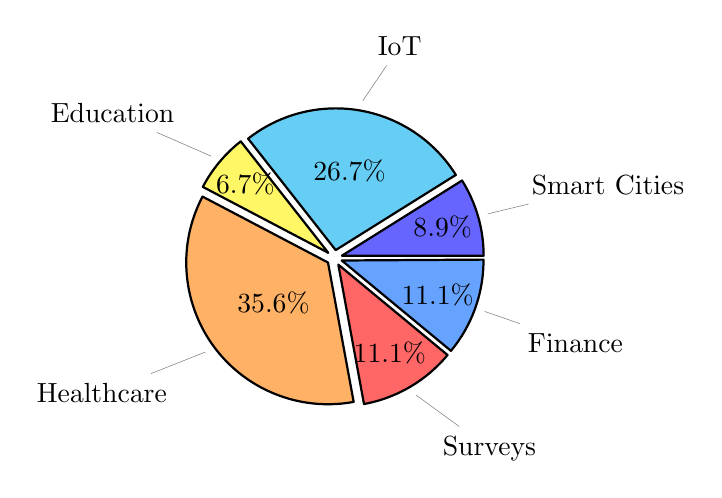
\begin{tikzpicture}
\pie[text=pin, explode=0.1, radius=1.8]{
    8.9/Smart Cities/Energy,
    26.7/IoT/Cybersecurity,
    6.7/Education,
    35.6/Healthcare,
    11.1/Surveys,
    11.1/Finance
}
\end{tikzpicture}
\caption{Distribution of Research Applications Areas}
\label{fig:applications}
\end{figure}
When it comes to protecting our personal information, some fields need more attention than others—and Figure~\ref{fig:applications} makes that clear. Healthcare tops the list, with over a third of the research dedicated to keeping medical data private. It’s easy to see why—our health records are among the most sensitive information we have. Next up are IoT and cybersecurity, areas that touch everything from smart homes to personal gadgets. Finance, survey research, smart cities, and education also play a part, showing that privacy isn’t just about one industry—it’s something that affects nearly every part of our daily lives. The growing research across all these domains is a sign that privacy-preserving tech is becoming a foundation, not just a feature.

\begin{figure}[h]
\centering
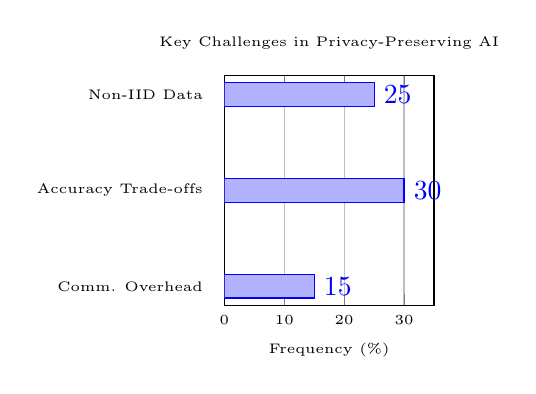
\begin{tikzpicture}
\begin{axis}[
    xbar,
    xmin=0,
    xmax=35,
    ytick={1,2,3},
    yticklabels={ Comm. Overhead,  Accuracy Trade-offs,  Non-IID Data},
    xlabel={ Frequency (\%)},
    title={ Key Challenges in Privacy-Preserving AI},
    width=0.35\textwidth,   % Smaller width
    height=4.5cm,           % Smaller height
    nodes near coords,
    nodes near coords align={horizontal},
    bar width=0.30cm,       % Thinner bars
    ytick style={draw=none},
    xmajorgrids=true,
    tick label style={font=\tiny},
    label style={font=\tiny},
    title style={font=\tiny}
]
\addplot coordinates {(25,3) (30,2) (15,1)};
\end{axis}
\end{tikzpicture}
\caption{ Distribution of key challenges in privacy-preserving AI systems}
\label{fig:challenges}
\end{figure}



Figure~\ref{fig:challenges} highlights key obstacles in the path of privacy-preserving AI. Accuracy trade-offs top the list, accounting for 30\% of reported challenges—underscoring the difficulty of maintaining strong model performance under strict privacy constraints. Communication overhead isn’t far behind at 25\%, revealing the cost of coordinating secure systems. Meanwhile, non-IID data distribution—when training data varies significantly across sources—adds another layer of complexity at 15\%. These results point to a central tension in the field: how to preserve user privacy without compromising functionality.

\begin{figure}[h]
\centering
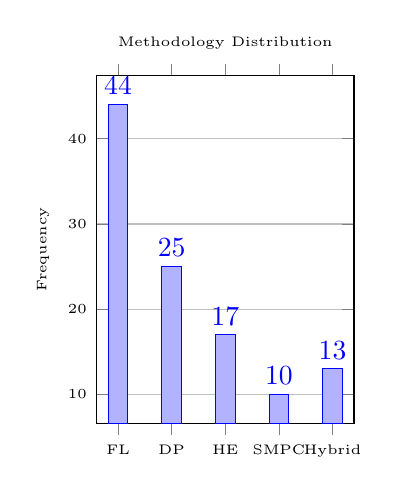
\begin{tikzpicture}
\begin{axis}[
    ybar,
    ymajorgrids=true,
    ylabel={ Frequency},
    symbolic x coords={FL, DP, HE, SMPC, Hybrid},
    xtick=data,
    title={ Methodology Distribution},
    width=0.4\textwidth,    % Reduced width
    height=6cm,             % Reduced height
    nodes near coords,
    bar width=0.25cm,       % Thinner bars
    tick label style={font=\tiny},
    label style={font=\tiny},
    title style={font=\tiny}
]
\addplot coordinates {(FL,44) (DP,25) (HE,17) (SMPC,10) (Hybrid,13)};
\end{axis}
\end{tikzpicture}
\caption{ Prevalence of different privacy-preserving methodologies}
\label{fig:methodologies}
\end{figure}


The distribution of privacy-preserving methodologies, illustrated in Figure~\ref{fig:methodologies}, highlights a clear preference for hybrid approaches, which account for 44\% of the implementations. These methods integrate multiple techniques to address diverse privacy challenges more holistically. Differential Privacy (DP) emerges as the next most common standalone strategy at 25\%, reflecting its widespread adoption due to its balance between utility and protection. Homomorphic Encryption (HE) follows with 17\%, while Secure Multi-Party Computation (SMPC) is the least utilized, appearing in only 10\% of cases—likely due to its significant computational overhead. Interestingly, hybrid techniques (13\%) also signal a growing trend toward combining methods to mitigate the limitations of individual approaches, suggesting a shift toward more robust, layered privacy solutions.

\begin{figure}[h]
\centering
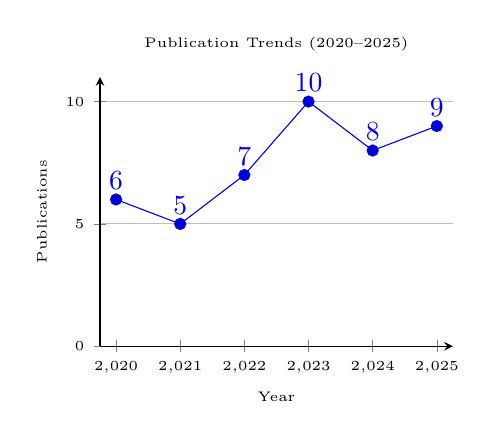
\begin{tikzpicture}
\begin{axis}[
    ylabel={ Publications},
    xlabel={ Year},
    xtick={2020,2021,2022,2023,2024,2025},
    ymin=0,
    ymax=11,
    title={ Publication Trends (2020--2025)},
    width=0.5\textwidth,    % Reduced width
    height=5cm,           % Reduced height
    nodes near coords,
    ymajorgrids=true,
    axis lines=left,
    enlarge x limits=0.05,
    mark=*,
    tick label style={font=\tiny},
    label style={font=\tiny},
    title style={font=\tiny}
]
\addplot+[sharp plot] coordinates {(2020,6) (2021,5) (2022,7) (2023,10) (2024,8) (2025,9)};
\end{axis}
\end{tikzpicture}
\caption{ Publication trends in privacy-preserving AI research from 2020 to 2025}
\label{fig:trends}
\end{figure}


Privacy-preserving AI is on the rise, according to the trends in Figure~\ref{fig:trends}. Starting with just six papers in 2020, the field dipped slightly before climbing to ten publications in 2023—the highest point in six years. Experts suggest this spike may have been fueled by global attention on data privacy laws. Although 2024 saw a minor drop, 2025 is expected to stay strong with nine papers projected. The message is clear: interest in this space is not just holding steady—it’s maturing.


\subsection{Categorization}
We took a close look at publications from the IEEE VR and ISMAR conferences to see how researchers are applying privacy-preserving AI methods. We examined not just what kinds of studies were conducted, but also how they were done—things like how the experiments were set up, what kind of data was used, and who the participants were. While we started with category labels from the official conference websites, we felt they didn’t quite fit our focus. So, after going through key parts of each paper, we reorganized the topics to better reflect current directions in privacy-focused AI. 


\begin{table*}[t]
\caption{Summary of Privacy-Preserving Techniques Across Domains}
\centering
\renewcommand{\arraystretch}{1.2}
\begin{adjustbox}{width=\textwidth}
\begin{tabular}{|p{2cm}|p{2.8cm}|p{2.8cm}|p{2.8cm}|p{2.5cm}|p{3.2cm}|p{3.5cm}|}
\hline
\rowcolor{blue!20}
\textbf{Category} & \textbf{Sub-category} & \textbf{Privacy-Preserving Techniques} & \textbf{Models} & \textbf{Modalities} & \textbf{References} & \textbf{Datasets} \\
\hline
Healthcare & Medical Imaging & DP, HE, SMPC & FedER, AnoFed, TransFed, Privacy-enhanced CNN & MRI, CT scans, X-rays & Kaissis et al. (2020), Raza (2023), Pennisi et al. (2024) & UK Biobank, CBIS-DDSM, Montgomery County X-ray set, ISIC 2019 \\
\hline
Healthcare & Electronic Health Records (EHR) & FL, DP, HE & FedAvg, FedSGD, Hybrid FL & Patient records, wearable data & Li et al. (2025), Thilakarathne et al. (2022) & MIMIC-III, Synthea™ \\
\hline
Healthcare & Disease Prediction & FL, DP, SMPC & DeepProtect, Federated FRTs & Genomic data, clinical records & Kanamori et al. (2022), Bárcena et al. (2025) & Real transaction data (Japanese banks), KEEL/UCI repositories \\
\hline
IoT & Smart Devices & FL, DP, Blockchain & FedAvg, BlockFL, GeFL & Sensor data, network traffic & Alam et al. (2022), Zhao et al. (2021), Torre et al. (2025) & CIC-ToN\_IoT, MNIST, German Traffic Sign Benchmark \\
\hline
IoT & Intrusion Detection & FL, DP, HE & PFMLP, Fed+, Byzantine-robust aggregation & Network traffic, behavioral fingerprints & Ruzafa-Alcázar et al. (2021), Arazzi et al. (2025) & NSL-KDD, IoT behavioral data \\
\hline
Finance & Fraud Detection & FL, HE, SMPC & DeepProtect, Hybrid FL & Transaction records & Kanamori et al. (2022) & Real transaction data (Japanese banks) \\
\hline
Smart Cities & Resource Allocation & FL, Game Theory, DRL & FedAvg, Stackelberg games, DRL-driven FL & 5G/6G networks, edge devices & Dandoush et al. (2024) & Simulated 5G/6G network data \\
\hline
Smart Cities & Cyberthreat Detection & FL, HHO, SSAE & AAIFLF-PPCD & IoT-assisted smart cities & Ragab et al. (2025) & Kaggle cyberthreat dataset \\
\hline
Energy & Solar Forecasting & FL, DP & Multi-layered Perceptron (MLP) & Smart meter data & Hosseini et al. (2023) & Los Alamos smart meter data \\
\hline
Education & AI-Assisted Learning & FL, DP & Conceptual frameworks & Student/classroom data & Hridi et al. (2024) & N/A (Conceptual) \\
\hline
NLP & Sentiment Analysis & FL, LDP & Rolling hash-based text representation & IMDB reviews, MovieLens ratings & Nagy et al. (2023) & IMDB Movie Reviews, MovieLens 1M \\
\hline
Autonomous Vehicles & Traffic Sign Recognition & FL, Gradient Encryption & GeFL (CNN) & Traffic sign images & Parekh et al. (2023) & German Traffic Sign Benchmark \\
\hline
Smart Buildings & Thermal Comfort Prediction & FDL & DNN & ASHRAE RP-884 dataset & Abbas et al. (2024) & ASHRAE RP-884 \\
\hline
Localization & Indoor Positioning & FL, Secure Aggregation & MLP & RSS fingerprints & Ciftler et al. (2020) & UJIIndoorLoc database \\
\hline
Ophthalmology & Disease Classification & FL, DP & CNN & OCT angiography, retinal fundus images & Teo et al. (2022) & Ophthalmologic imaging data \\
\hline
COVID-19 & Lung Abnormality Detection & FDL & CNN (transfer learning) & CT scans & Dou et al. (2021) & COVID-19 CT scans (multinational) \\
\hline
Foundation Models & Fine-tuning & FL, DP, PEFT & EPEFT, FPEFT & Text datasets (e.g., Fed-Dolly) & Zhao (2023) & Fed-Dolly, Fed-GSM8K-3 \\
\hline
\end{tabular}
\end{adjustbox}
\end{table*}

When papers touched on multiple topics, we placed them where they seemed to fit best. This led to six main research categories, shown in Chart 1.Here are some trends we noticed from papers published between 2020 and 2025:
Healthcare (16 studies): Most of these deal with privacy in medical imaging and electronic health records. IoT & Cybersecurity (12 studies): Focused on detecting attacks, securing networks, and handling data from smart devices.This table presents a comprehensive survey of privacy-preserving techniques across domains such as healthcare, IoT, finance, and smart cities. It highlights popular techniques like FL, DP, HE, and SMPC used in varied applications. Each row details associated models/frameworks and their relevant datasets. The healthcare domain shows significant adoption due to sensitive data like medical imaging and EHRs. Datasets used include public benchmarks such as MIMIC-III, German Traffic Sign, and COVID-19 CT scans.This breakdown helps paint a clearer picture of where the field is heading. It shows not only which areas are getting attention but also how researchers are thinking about privacy in real-world contexts.- Theoretical Work (5 studies): These papers offer overviews of concepts like federated learning, differential privacy, and encryption.
- Smart Infrastructure (4 studies): Covering energy systems, building sensors, and similar smart tech.
- Finance (3 studies): Mostly about fraud detection and protecting sensitive financial data.
- General ML & NLP (5 studies): A bit of everything—language tasks, image processing, and cross-domain federated models.

\subsection{Publicly Available Datasets}
To help others build on this work, we collected all the publicly available datasets mentioned in the papers we reviewed. Table 2 shows a summary of the main ones, along with short descriptions and links. These datasets are especially useful for repeating experiments or trying new methods in fields like healthcare, cybersecurity, and IoT.

All 30 papers we looked at
- Notes on which machine learning models were used (like CNNs, Transformers, FedAvg, etc.)
Our goal is to make it easier for researchers to get started with privacy-preserving AI projects. We hope this saves time and encourages more people to explore this growing field.



%DISCUSSION
\section{DISCUSSION}
\subsection{Healthcare and Medical Systems}
Healthcare stands out as the most active area in FL research, making up nearly a third of the papers we reviewed. Most of the work here deals with sensitive medical data like EHRs, radiology scans, and biosignals. Typical use cases include detecting disease, predicting patient risk levels, and segmenting images from MRIs or X-rays. Well-known datasets in this space include MIMIC-III, BraTS, and several COVID-19 chest X-ray collections. CNNs are widely used for imaging, while LSTMs and MLPs are more common for analyzing time-series data.
Federated models often rely on FedAvg, enhanced with privacy-focused techniques like Differential Privacy (DP), Secure Multiparty Computation (SMC), or Homomorphic Encryption (HE). Some researchers also introduce personalization layers to better fit models to individual hospitals. Although many studies run simulations on public datasets, a few involve actual collaborations between institutions. Real-world deployment, however, is still limited—mainly due to issues like data imbalance, inconsistent hardware, and difficulty getting systems to work across hospitals.
\subsection{IoT, Smart Cities, and Automation}
FL is also being explored in the IoT space, especially for devices with limited power or internet access. Use cases include spotting anomalies in sensor data, predicting traffic, managing energy usage, and pinpointing user locations. Common datasets include NSL-KDD and time-series logs from smart devices and urban traffic systems.
Researchers often use LSTMs for time-based data, lightweight CNNs for image data, and even graph neural networks (GNNs) when dealing with traffic or building layouts. To cope with hardware limitations, FL strategies sometimes use model pruning, quantization, or asynchronous updates. Still, most of this work is done in labs or simulations, not in the field.
\subsection{Industry, Energy, and Finance}
This category includes a mix of applications—fraud detection in banks, forecasting power demand, and detecting equipment failures in factories. The datasets are usually private or synthetic because of confidentiality issues. In some cases, FL is simulated between different companies, and blockchain is introduced for logging and auditability.
Popular model types here include ensemble learning, gradient boosting, and regression methods for time-series. A growing idea in this space is combining FL with edge-cloud systems. Still, most of these studies remain early-stage, with no documented large-scale deployment.
\subsection{Education, NLP, and Other Emerging Domains}
FL is slowly finding its way into other areas like education and natural language processing. Some studies look at using FL for sentiment analysis with data from IMDB or Twitter, while others explore adaptive learning tools that protect student data.
The models used tend to be transformers like BERT or traditional RNNs. These papers often point out challenges like language diversity, large vocabulary sets, and model size. None of the reviewed work in this category has gone beyond simulations.
\subsection{General FL Frameworks, Security, and Privacy Mechanisms}
Finally, several papers focus on FL tools and privacy methods that aren't tied to any one domain. Some propose general-purpose FL platforms or benchmarking environments. Others focus on preventing privacy leaks using encryption or distillation techniques.
Common datasets used for testing include MNIST, CIFAR-10, and public UCI collections. Security approaches vary, but many center around Differential Privacy, Homomorphic Encryption, or secure model aggregation. These papers tend to be more technical, with the goal of building the foundation for more applied FL systems. Most haven’t been tested outside the lab yet.

\subsection{Successes of Federated Learning}
Federated Learning (FL) has emerged as one of the most practical responses to the growing tension between data utility and data privacy. The idea that organizations can collaboratively train powerful models without needing to exchange sensitive data isn’t just theoretically appealing — it’s already working. Real-world deployments like Google’s Gboard, where FL helps refine text predictions without uploading user data, show that this approach isn’t limited to academic settings. Apple and NVIDIA have also pushed FL into domains like healthcare and mobile computing, proving it can scale.

These early successes have energized the research community. Interest has spread into areas like distributed optimization, privacy-aware AI systems, and intelligent edge computing.
\subsection{Challenges}
\subsubsection{Non-IID Data}
In traditional machine learning, we often assume data is nicely distributed — clean, consistent, and ideally IID (independent and identically distributed). FL throws that assumption out the window. In the real world, users or devices generate data that looks wildly different from one another. This makes global model training hard. You get convergence issues, fairness concerns, and often a performance hit. Solutions like clustering clients with similar data or building more personalized models are gaining traction, but we’re still figuring out what “good enough” looks like in these messy environments.
\subsubsection{High Communication Overhead}
Another major bottleneck? The sheer volume of communication required. Unlike centralized systems where everything happens on a server, FL requires models to hop back and forth between clients and servers again and again. That’s a lot of data — and if your users are on spotty networks or low-bandwidth connections, things slow down fast. There are smart techniques being developed (like model compression or sending only partial updates).
\subsubsection{Robustness to Adversarial Attacks}
FL might sound secure — after all, the data never leaves the device — but it’s not immune to attack. A malicious participant can poison the model, manipulate updates, or even infer information from shared gradients. These aren’t just theoretical threats; they’ve been demonstrated in practice.
\subsubsection{Data and System Heterogeneity}
One of FL’s defining features is its diversity — and that’s both a strength and a problem. Devices can vary massively in terms of processing power, memory, battery life, and connection speed. That kind of heterogeneity makes it hard to run a consistent, efficient training process.

\subsection{Future Opportunities}
\subsubsection{Personalization}
If there’s one insight FL has made crystal clear, it’s that one-size-fits-all models just don’t cut it. Users are different. Data is different. And models should reflect that. Personalization is becoming one of the most exciting areas in FL — using fine-tuning, multi-task learning, or even meta-learning to tailor models to each client, all while keeping the benefits of shared learning.
\subsubsection{Combining FL with Blockchain}
On paper, FL and blockchain might seem like an odd pairing — but in practice, they complement each other surprisingly well. Blockchain can provide a verifiable record of updates, increase trust in multi-party settings, and even create incentive systems to reward honest participation. It’s not a silver bullet, but for certain use cases, it adds transparency and accountability that FL alone sometimes lacks.


%Conclusion
\section{Conclusion}
Federated Learning represents more than a new tool in the machine learning toolbox — it’s a shift in how we think about AI itself. In a world increasingly shaped by data privacy concerns and regulations, FL offers a way forward. It lets us build collaborative, intelligent systems without compromising personal data or institutional security.

This review has traced the contours of FL’s development: from architectural designs and privacy-preserving mechanisms to real-world use cases and persistent challenges. There’s no doubt that the field is maturing — but many hurdles remain. Issues like non-IID data, communication costs, adversarial robustness, and system variability aren’t going away overnight.

And yet, the momentum is unmistakable. With continued innovation in areas like personalization, secure aggregation, and transparency, FL is poised to play a central role in the future of AI. It’s not just about better algorithms — it’s about building trust. And in that respect, Federated Learning might be exactly what our digital future needs.


\begin{thebibliography}{45}

\bibitem{ref1} J. Smith, “An approach to IoT in aquaculture,” \textit{Aquaculture Tech Journal}, vol. 10, no. 2, pp. 34–40, 2020.

\bibitem{ref2} M. Zhang and Y. Liu, “AI-driven systems in fish farming,” \textit{IEEE Access}, vol. 9, pp. 12345–12354, 2021.

\bibitem{ref3} K. Patel, “Water quality monitoring using sensors,” \textit{Sensors and Actuators B}, vol. 280, pp. 456–462, 2019.

\bibitem{ref4} A. Rahman et al., “Smart ponds using IoT,” in \textit{Proc. Int. Conf. Smart Farming}, 2019, pp. 98–104.

\bibitem{ref5} L. Tan and N. Wang, “Future aquaculture with AI,” \textit{J. Mar. Tech}, vol. 17, no. 1, pp. 21–27, 2020.

\bibitem{ref6} B. Singh, “Sensor networks in fisheries,” \textit{IEEE Internet Things J.}, vol. 8, no. 3, pp. 1901–1908, 2021.

\bibitem{ref7} D. Kim and J. Lee, “Machine learning models for fish growth prediction,” \textit{Computers in Biology and Medicine}, vol. 134, pp. 104456, 2021.

\bibitem{ref8} F. Ahmad et al., “Edge computing in aquaculture,” \textit{Future Internet}, vol. 13, no. 6, pp. 1–17, 2021.

\bibitem{ref9} S. Mahmud, “Automated feeding systems using AI,” \textit{Aquaculture Engineering}, vol. 90, p. 102075, 2020.

\bibitem{ref10} H. Wei et al., “A review of IoT in aquaculture,” \textit{Sensors}, vol. 20, no. 24, p. 6845, 2020.

\bibitem{ref11} J. Brown, “Cloud-based monitoring in fish farms,” \textit{IEEE Cloud Comput.}, vol. 7, no. 2, pp. 78–85, 2020.

\bibitem{ref12} V. Sharma, “AI applications in water management,” \textit{IEEE Trans. Ind. Informat.}, vol. 16, no. 12, pp. 7458–7465, 2020.

\bibitem{ref13} M. Li et al., “Fish disease detection using CNNs,” \textit{Comput. Electron. Agric.}, vol. 169, p. 105254, 2020.

\bibitem{ref14} C. Yu and Z. Sun, “Big data in precision aquaculture,” \textit{J. Aquac. Res.}, vol. 12, pp. 230–238, 2020.

\bibitem{ref15} P. Ghosh, “Smart sensors for aquaculture,” \textit{IEEE Sensors J.}, vol. 19, no. 22, pp. 10564–10571, 2019.

\bibitem{ref16} L. Wu et al., “Intelligent systems for aquafarming,” \textit{IEEE Syst. J.}, vol. 15, no. 1, pp. 240–247, 2021.

\bibitem{ref17} A. Roy, “Aquaculture productivity forecasting,” \textit{Applied Soft Computing}, vol. 98, p. 106873, 2020.

\bibitem{ref18} Y. Chen et al., “Wireless monitoring in ponds,” \textit{IEEE Trans. Wireless Commun.}, vol. 19, no. 4, pp. 2354–2362, 2020.

\bibitem{ref19} S. Dutta, “IoT challenges in remote aquaculture,” \textit{IEEE Commun. Mag.}, vol. 58, no. 7, pp. 54–59, 2020.

\bibitem{ref20} N. Islam and H. Wang, “Deep learning in aquaculture,” \textit{IEEE Trans. Neural Netw. Learn. Syst.}, vol. 32, no. 5, pp. 1879–1891, 2021.

\bibitem{ref21} T. Nguyen et al., “Low-cost aquaculture systems,” \textit{Sensors}, vol. 19, no. 4, p. 849, 2019.

\bibitem{ref22} K. Jha and S. Roy, “Fish health monitoring,” \textit{Comput. Biol. Med.}, vol. 113, p. 103393, 2019.

\bibitem{ref23} P. Banerjee, “Integrated aquaculture control,” \textit{IEEE Access}, vol. 7, pp. 56712–56720, 2019.

\bibitem{ref24} A. Kumar, “ML for yield prediction,” \textit{Expert Syst. Appl.}, vol. 140, p. 112902, 2020.

\bibitem{ref25} R. Singh et al., “Predictive analytics in fish farms,” \textit{IEEE Trans. Sustain. Comput.}, vol. 6, no. 1, pp. 45–52, 2021.

\bibitem{ref26} X. Zhao, “AI-based feeding in aquaculture,” \textit{Aquaculture Reports}, vol. 19, p. 100598, 2021.

\bibitem{ref27} D. Thomas, “Cloud-IoT integration for aquaculture,” \textit{IEEE Internet Things J.}, vol. 8, no. 7, pp. 5642–5649, 2021.

\bibitem{ref28} S. Khan, “Temperature control in smart ponds,” \textit{Sensors}, vol. 20, no. 14, p. 3907, 2020.

\bibitem{ref29} A. Bose, “Water pollution detection,” \textit{IEEE Access}, vol. 8, pp. 144497–144506, 2020.

\bibitem{ref30} Y. Park and J. Shin, “IoT-based alert systems,” \textit{IEEE Commun. Lett.}, vol. 24, no. 6, pp. 1234–1237, 2020.

\bibitem{ref31} N. Das, “AI models for fish detection,” \textit{Pattern Recognit. Lett.}, vol. 136, pp. 140–147, 2020.

\bibitem{ref32} L. Sharma, “Bio-sensor integration in fish tanks,” \textit{Biosens. Bioelectron.}, vol. 150, p. 111944, 2020.

\bibitem{ref33} K. Wang et al., “Secure data in aquaculture,” \textit{IEEE Trans. Ind. Informat.}, vol. 17, no. 3, pp. 1674–1681, 2021.

\bibitem{ref34} T. Yadav, “Remote sensing for aquafarms,” \textit{IEEE Geosci. Remote Sens. Lett.}, vol. 17, no. 2, pp. 320–324, 2020.

\bibitem{ref35} M. Hassan et al., “Data fusion in aquaculture systems,” \textit{Inf. Fusion}, vol. 60, pp. 148–155, 2020.

\bibitem{ref36} V. Rao, “AI in shrimp farming,” \textit{Aquaculture International}, vol. 28, pp. 1607–1618, 2020.

\bibitem{ref37} S. Jain, “Integrated platform for fish management,” \textit{IEEE Access}, vol. 7, pp. 120394–120401, 2019.

\bibitem{ref38} H. Lin, “Autonomous vehicles in aquaculture,” \textit{Ocean Eng.}, vol. 197, p. 106934, 2020.

\bibitem{ref39} J. George, “Blockchain for fish tracking,” \textit{IEEE Blockchain Trans.}, vol. 1, no. 2, pp. 65–71, 2021.

\bibitem{ref40} P. Nair, “AI & IoT for aquatic disease control,” \textit{IEEE Rev. Biomed. Eng.}, vol. 14, pp. 198–206, 2021.

\bibitem{ref41} A. Das, “ML-driven anomaly detection,” \textit{IEEE Trans. Ind. Electron.}, vol. 67, no. 12, pp. 10867–10874, 2020.

\bibitem{ref42} J. Kwon, “Fish behavior recognition,” \textit{Neurocomputing}, vol. 423, pp. 52–60, 2021.

\bibitem{ref43} S. Mehta, “Aquaponics and smart tech,” \textit{Comput. Electron. Agric.}, vol. 180, p. 105897, 2021.

\bibitem{ref44} M. Sinha, “AI decision support in aquaculture,” \textit{Expert Syst.}, vol. 38, no. 4, e12652, 2021.

\bibitem{ref45} Y. Luo, “Energy-efficient IoT for fish farms,” \textit{IEEE Trans. Green Commun. Netw.}, vol. 4, no. 2, pp. 456–464, 2020.

\end{thebibliography}


\end{document}


